\documentclass[11pt,a4paper,twoside]{article}

% LaTeX-Umsetzung der "Richtlinien für Projekt- und Diplomarbeiten"
% der LFE Medieninformatik, LMU München. (Autor: Richard Atterer, 27.9.2006, 23.10.2007), Bug-Fixing Mark Kaczkowski (23.6.2008)
\usepackage[backend=biber, style=ieee]{biblatex}
\usepackage{makecell}
\addbibresource{sample.bib}
\usepackage[T1]{fontenc} % sonst geht \hyphenation nicht mit Umlauten
\usepackage{booktabs}
\usepackage{listings}
%\usepackage[latin1]{inputenc} % man kann schreiben äöüß, statt "a"o"u"s
\usepackage[utf8]{inputenc} % wie oben, aber UTF-8 als Encoding statt ISO-8859-1 (latin1)
%\usepackage[ngerman,english]{babel} % deutsche Trennregeln, "Inhaltsverzeichnis" etc.
% \usepackage{ngerman} % Alternative zum Babel-Paket oben
% \usepackage{mathptmx} % Times-Roman-Schrift (auch für mathematische Formeln)
\usepackage{tgpagella}
% Zum Setzen von URLs
\usepackage{color}
\definecolor{darkred}{rgb}{.25,0,0}
\definecolor{darkgreen}{rgb}{0,.2,0}
\definecolor{darkmagenta}{rgb}{.2,0,.2}
\definecolor{darkcyan}{rgb}{0,.15,.15}
\usepackage[plainpages=false,bookmarks=true,bookmarksopen=true,colorlinks=true,
  linkcolor=darkred,citecolor=darkgreen,filecolor=darkmagenta,
  menucolor=darkred,urlcolor=darkcyan]{hyperref}
\usepackage{caption}
\usepackage{subcaption}

% pdflatex: Bilder in den Formaten .jpeg, .png und .pdf
% latex: Bilder im .eps-Format
\usepackage{graphicx}

\usepackage{subfiles}

\usepackage{fancyhdr} % Positionierung der Seitenzahlen
\fancyhead[LE,RO,LO,RE]{}
\fancyfoot[CE,CO,RE,LO]{}
\fancyfoot[LE,RO]{\Roman{page}}
\renewcommand{\headrulewidth}{0pt}
\setlength{\headheight}{13.6pt} % behebt headheight Warning

% Korrektes Format für Nummerierung von Abbildungen (figure) und
% Tabellen (table): <Kapitelnummer>.<Abbildungsnummer>
\makeatletter
\@addtoreset{figure}{section}
\renewcommand{\thefigure}{\thesection.\arabic{figure}}
\@addtoreset{table}{section}
\renewcommand{\thetable}{\thesection.\arabic{table}}
\makeatother

\sloppy % Damit LaTeX nicht so viel über "overfull hbox" u.Ä. meckert

% Ränder
\addtolength{\topmargin}{-16mm}
\setlength{\oddsidemargin}{25mm}
\setlength{\evensidemargin}{35mm}
\addtolength{\oddsidemargin}{-1in}
\addtolength{\evensidemargin}{-1in}
\setlength{\textwidth}{15cm}
\addtolength{\textheight}{34mm}
%______________________________________________________________________

\begin{document}

\pagestyle{empty} % Vorerst keine Seitenzahlen
\pagenumbering{alph} % Unsichtbare alphabetische Nummerierung

\begin{center}
\textsc{Ludwig-Maximilians-Universität München}\\
Department ``Institut für Informatik''\\
Lehr- und Forschungseinheit Medieninformatik\\
Prof.\ Dr.\ Heinrich Hußmann

\vspace{5cm}
{\large\textbf{Masterarbeit}}\vspace{.5cm}

{\LARGE Increasing Robustness of Facial Expression Recognition against Speech}\vspace{1cm}

{\large Marcel Baur}\\\href{mailto:marcel.baur@campus.lmu.de}{marcel.baur@campus.lmu.de}

\end{center}
\vfill

\begin{tabular}{ll}
Bearbeitungszeitraum: & 1. 1. 2021 bis 2. 7. 2021\\
Betreuer: & Matthias Schmidmaier\\
Externer Betreuer: & Ciprian Corneanu\\
Verantw. Hochschullehrer: & Prof. Hußmann
\end{tabular}
%______________________________________________________________________

\clearpage
% \section*{Zusammenfassung}

% Kurzzusammenfassung der Arbeit, maximal 250 Wörter.

% \selectlanguage{english}
\section*{Abstract}

Short abstract of the work, maximum of 250 words.

% \selectlanguage{ngerman}
\clearpage
\section*{Aufgabenstellung}

Kopie der Original-Aufgabenstellung

\vfill % Sorgt dafür, dass das Folgende an das Seitenende rutscht

\noindent Ich erkläre hiermit, dass ich die vorliegende Arbeit
selbstständig angefertigt, alle Zitate als solche kenntlich gemacht
sowie alle benutzten Quellen und Hilfsmittel angegeben habe.

\bigskip\noindent München, 02.07.2021

\vspace{4ex}\noindent\makebox[7cm]{\dotfill}

%______________________________________________________________________

\cleardoublepage
\pagestyle{fancy}
\pagenumbering{roman} % Römische Seitenzahlen
\setcounter{page}{1}

% Inhaltsverzeichnis erzeugen
\tableofcontents

%Abbildungsverzeichnis erzeugen - normalerweise nicht nötig
%\cleardoublepage
%\listoffigures
%______________________________________________________________________

\cleardoublepage

% Arabische Seitenzahlen
\pagenumbering{arabic}
\setcounter{page}{1}
% Geändertes Format für Seitenränder, arabische Seitenzahlen
\fancyhead[LE,RO]{\rightmark}
\fancyhead[LO,RE]{\leftmark}
\fancyfoot[LE,RO]{\thepage}

% \chapter{Introduction}
\section{Introduction}
\label{sec:intro}

The study of detecting and quantifying human emotion has been a topic for many years. Going back to 1894, William James proclaimed that emotion is a result of our actions \cite{james1948emotion}. More important though was his idea that emotion correlates to feeling \cite{james2007principles}. Emotions themselves are induced by stimuli, which excite the human subject and thus propagates to bodily change. According to Izard, the core theories that view cognitive and sensory processes as emotional activators can be followed back to James \cite{izard1990substrates}.

Going forward several years into the mid-90s, Picard consolidated ideas of computing and measuring affect in her 1995 essay, coining the term Affective Computing \cite{picard2000affective}. A subfield of affective computing is based around recognising affective states from facial expressions. Much of the progress in this field bases its research around several axiomatic assumptions, one of which being that all facial movements are induced by emotion. This is especially problematic if the analysed subject is speaking, since the act of talking also triggers facial movement and thus introduces noise into the input data. 

In this thesis, we want to find ways to make existing facial expression recognition models more robust towards talking subjects. We will analyse how humans detect emotion when confronted with speaking people (Chapter \ref{sec:human}), and try to include those findings in our models (Chapter \ref{sec:models}). We further benchmark our models against inputs of different languages, and speech acts that are more akin to those in the real world (Chapter \ref{sec:data}).

We conclude our work with an analysis of the different modalities of our models, and give an outlook into further research towards a more robust framework of facial emotion recognition that contextualises speech.

\begin{figure}
    \centering
    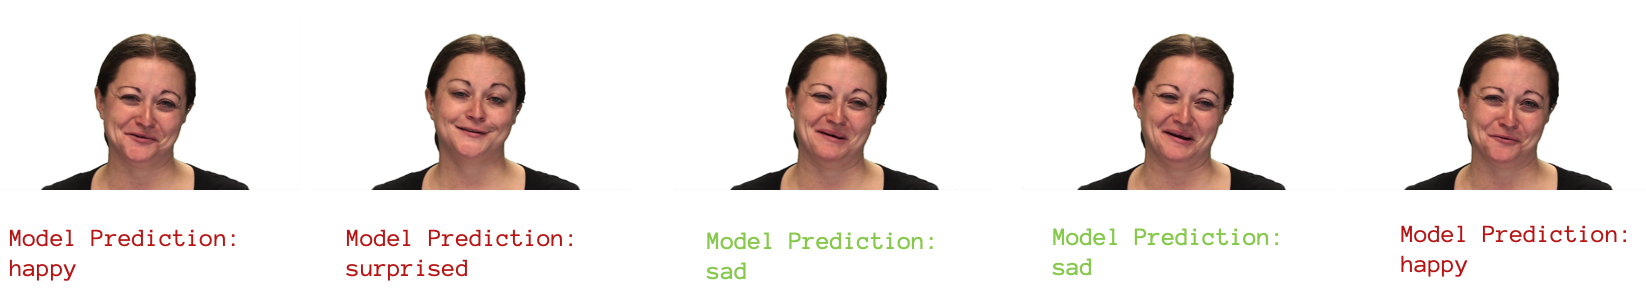
\includegraphics[width=0.8\textwidth]{res/modelex.png}
    \caption{An example of a model mislabeling a speaking subject talking while expressing a \texttt{sad} emotion \cite{livingstone2018ryerson}. Ideally, all frames, or the collection of frames, would be correctly categorized as \texttt{sad}.}
    \label{fig:mislabel}
\end{figure}
\section{Related Work}
\label{sec:related}
\subsection{Artificial Intelligence Techniques - Neural Networks}
\label{sub:aiml}
In this section we will describe common Artificial Intelligence (AI) techniques used in models for  facial expression recognition (Section \ref{sub:rw_fer}).
\subsubsection{Neural Networks}
A \emph{Neural Network NN} is built with many \emph{neurons}, which are connected by \emph{activators} that have a \emph{weight}. These neurons are located in many layers which give structure to the NN \cite{schmidhuber2015deep}. The first layer of the NN is the so-called \emph{input layer}, which acts as the entry point for the data that is to be analysed. The last layer is defined as the \emph{output layer}. It contains the information about the estimation that the NN has made. The in-between layers are called \emph{hidden layers}.

A NN can also be represented as a very complex function $f(x) = y$, where $x$ represents the input, and $y$ the computed output (the prediction).

Shallow NN consist of few hidden layers, and have been a topic for a long time. The discovery of \emph{backpropagation} allowed the development of NNs with many hidden layers, called \emph{Deep Neural Networks DNN} \cite{schmidhuber2015deep}.

\subsubsection{Convolutional Neural Networks CNN}
CNNs lend themselves well to tasks in \emph{Computer Vision CV} \cite{albawi2017understanding}. Most importantly, they reduce the amount of parameters, while also emphasizing locality and context of the input information. This enables edge detection, shape detection, and object detection in successive layers of a deep CNN, which will be especially helpful in models (Section \ref{sec:models}) that analyse faces and their active Action Units (Section \ref{subsub:au}).

Subsequent convolutional layers, coupled with pooling layers, enable the detection of more and more complex structures. While the initial layers might detect straight edges, the following layers will recognize compound structures, and ultimately features like raised eyebrows (AU 1 and/or AU 2).

\subsubsection{Temporal Neural Networks with Gated Recurrent Units GRU}
The previously described NNs can be described as \emph{feedforward} NNs. The direction of information flow is linearly through input, hidden and to the output layer. This can be contrasted with \emph{feedback} NNs, that have mechanisms that allow for 'memory' in a NN \cite{wang2003artificial}. These \emph{Recurrent Neural Networks RNN} enable the analysis of temporal data.

A concrete implementation for a temporal recurrent layer are \emph{Gated Recurrent Units GRU} proposed by Cho et al. \cite{cho2014properties} \cite{chung2014empirical}. GRUs act similarly to \emph{Long Short Term Memory LSTM} \cite{hochreiter1997lstm} layers, while removing memory gates \cite{chung2014empirical}. Empirical research has shown that GRUs can be more performant than LSTMs in less frequent datasets \cite{gruber2020gru}.

\subsection{Emotional Models from Facial Expression}
\label{sub:rw_fer}
\subsubsection{Categorical Model}
One of the most recognized ways to separate emotional states in non-verbal communication is presented by Paul Ekman \cite{ekman1987universals} \cite{ekman2013emotion}. His research postulates a cross-cultural agreement in judging facial expressions \cite{ekman1987universals}. Basic emotion theory assumes a fixed amount of human emotions, which is also believed and postulated by Ekman and Russell \cite{ekman1992basic} \cite{russell2006}. Ekman proposes a split into seven categories: anger, happiness, surprise, sadness, fear, disgust and contempt. He later consolidated them down to six, removing contempt. 

\subsubsection{Dimensional Model}

Dimensional systems use a set of dimensions, \emph{valence}, \emph{arousal} and in some cases \emph{dominance} to estimate the affective state of a person. James A. Russell introduced the two dimensional circumplex model of affect \cite{russell1980circumplex}, where he mapped emotions in the valence-arousal space. Valence represents the (un-)pleasantness of an affective state, and arousal represents the activation. \cite{posner2005circumplex}. The emotions from the categorical have their place in this dimensional field, e.g. happy having a high score for valence and arousal.

\begin{figure}
    \centering
    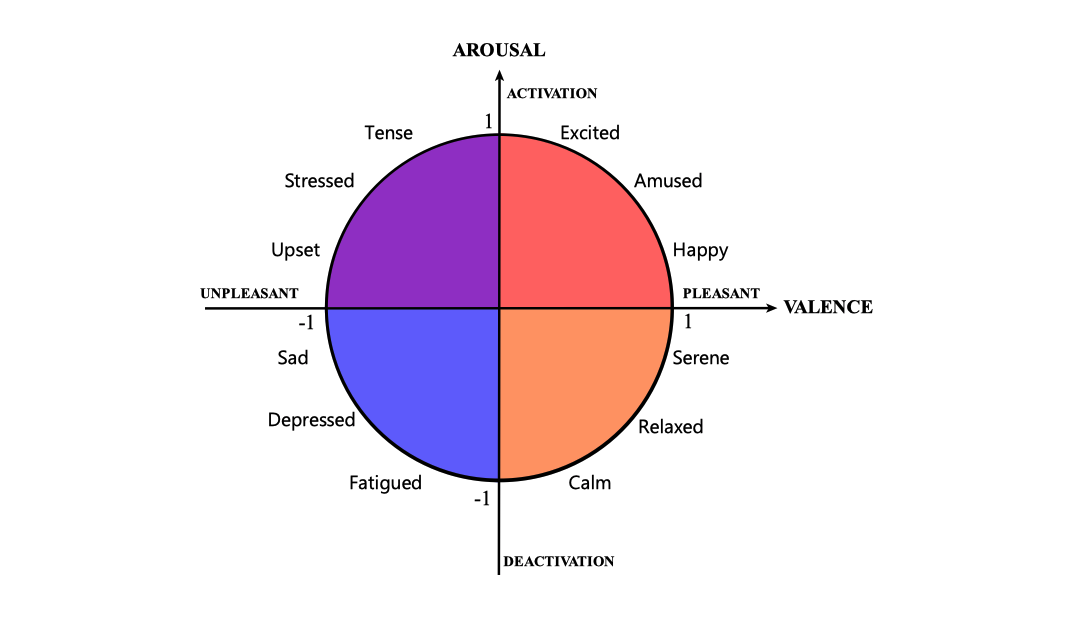
\includegraphics[width=0.8\textwidth]{res/circumplex.png}
    \caption{The circumplex model of affect with the valence and arousal axis with selected emotions. \cite{russell1980circumplex} \cite{pourmirzaei2021an}}
    \label{fig:circumplexImg}
\end{figure}

\subsubsection{Action Units}
\label{subsub:au}

Introduced by Hjortsjö \cite{hjortsjo1969man} and further refined by Ekman \cite{friesen1978facial}, the \emph{Facial Action Coding System FACS} tries to separate and classify facial movements that lead to distinct facial expressions. Combinations of the 28 \emph{Action Units AUs} can then be used to describe an affective expression.

\begin{table}[]
    \centering
    \begin{tabular}{c|c}
       \textbf{Emotion}  & \textbf{Action Units} \\ \hline
        Happy & 12, 25 \\
        Sad & 4, 15 \\
        Fearful & 1, 4, 20, 25 \\
        Angry & 4, 7, 24 \\
        Surprised & 1, 2, 25, 26 \\
        Disgusted & 9, 10, 17
    \end{tabular}
    \caption{The basic emotions with their corresponding prototypical AUs \cite{fabian2016emotionet}}
    \label{tab:emotionAUs}
\end{table}

\subsection{Automatic Facial Emotion Recognition}
Facial Emotion Recognition FER can be divided into two different groups: conventional and Deep-Learning-based. \cite{ko2018brief}

Conventional FER systems work in a pipeline that consists of three steps: face detection, feature extraction and expression classification \cite{ko2018brief}.

The deep learning approach has established itself as the state-of-the-art method for FER models. In contrast to the handcrafted conventional pipeline, the more modern approach enables an end-to-end learning method \cite{ko2018brief}. The most prominent model-type in FER is the convolutional neural network CNN. CNN-based networks offer themselves very well to image processing, which make them a great candidate for FER systems. 

Deep learning models can further be divided into two categories. The first one outputs emotions directly from the model \cite{ebrahimi2015recurrent} \cite{kim2017multi} \cite{jung2015joint}, where the second one classifies AU activations, from which emotions can be deduced \cite{breuer2017deep} \cite{zhao2016deep} \cite{chu2017learning}. 

\subsection{Phonemes and Visemes}
The content of an act of speech can be segmented into words, syllables, and \emph{phonemes} \cite{savin1970nonperceptual}. Languages differ in their amount of phonemes, with the New Guinean language Rotokas having 11, whereas the Namibias !Xóõ is using 160. English, the primary language we're be looking at in this thesis, has 37-41 phonemes, differing by dialect \cite{Hayes2009}. Phonemes are very important in FER. A speaking subjects face, and activated AUs, will be influenced by the lexical content of their speech, which is defined by the current phoneme. The face of a person in the act of pronouncing a phoneme will have a certain look to it. Several phonemes can be grouped together based on the distinct look they produce. These groups are called \emph{visemes}. There are several different phoneme-to-viseme mappings in research, with no concrete agreement on a 'best mapping' \cite{cappelletta2012viseme}.

Visemes are particularly interesting for us, since our research is purely based in the visual domain. Differences between phonemes that are purely audiocentric are of no relevance for us. A viseme mapping reduces the categories for visually based lexical content, which makes building and training models easier.
% \chapter{Research}

\section{Human FER during Speech}
\label{sec:human}
Given the limitations of detecting emotion in speaking faces, we look at the human ability of categorizing affective state. The CREMA-D corpus \cite{cao2014crema} includes aggregated results of the ratings collected from crowd-sourced labellers. These already give insights in human biases when categorizing emotion in talking subjects.

The videos in the CREMA-D corpus were acted and scripted. The actors were given a sentence and were tasked to speak that sentence in a given emotion. Annotators later evaluated these videos in three different modes:

\begin{enumerate}
    \item Audio only
    \item Video only
    \item Audio and Video
\end{enumerate}

We focus on the video-only task, since our models will also be only in the visual domain. Results of the analysis show some initially interesting results. Depending on the emotion, the annotators accuracy are significantly different. Videos on a happy emotion were labelled correctly 88\% of the time, whereas sad videos only had an accuracy of 32\% (Figure \ref{fig:crema_results}). The overall accuracy of the video-only annotation stands at 58.2\%.

\begin{figure}
    \centering
    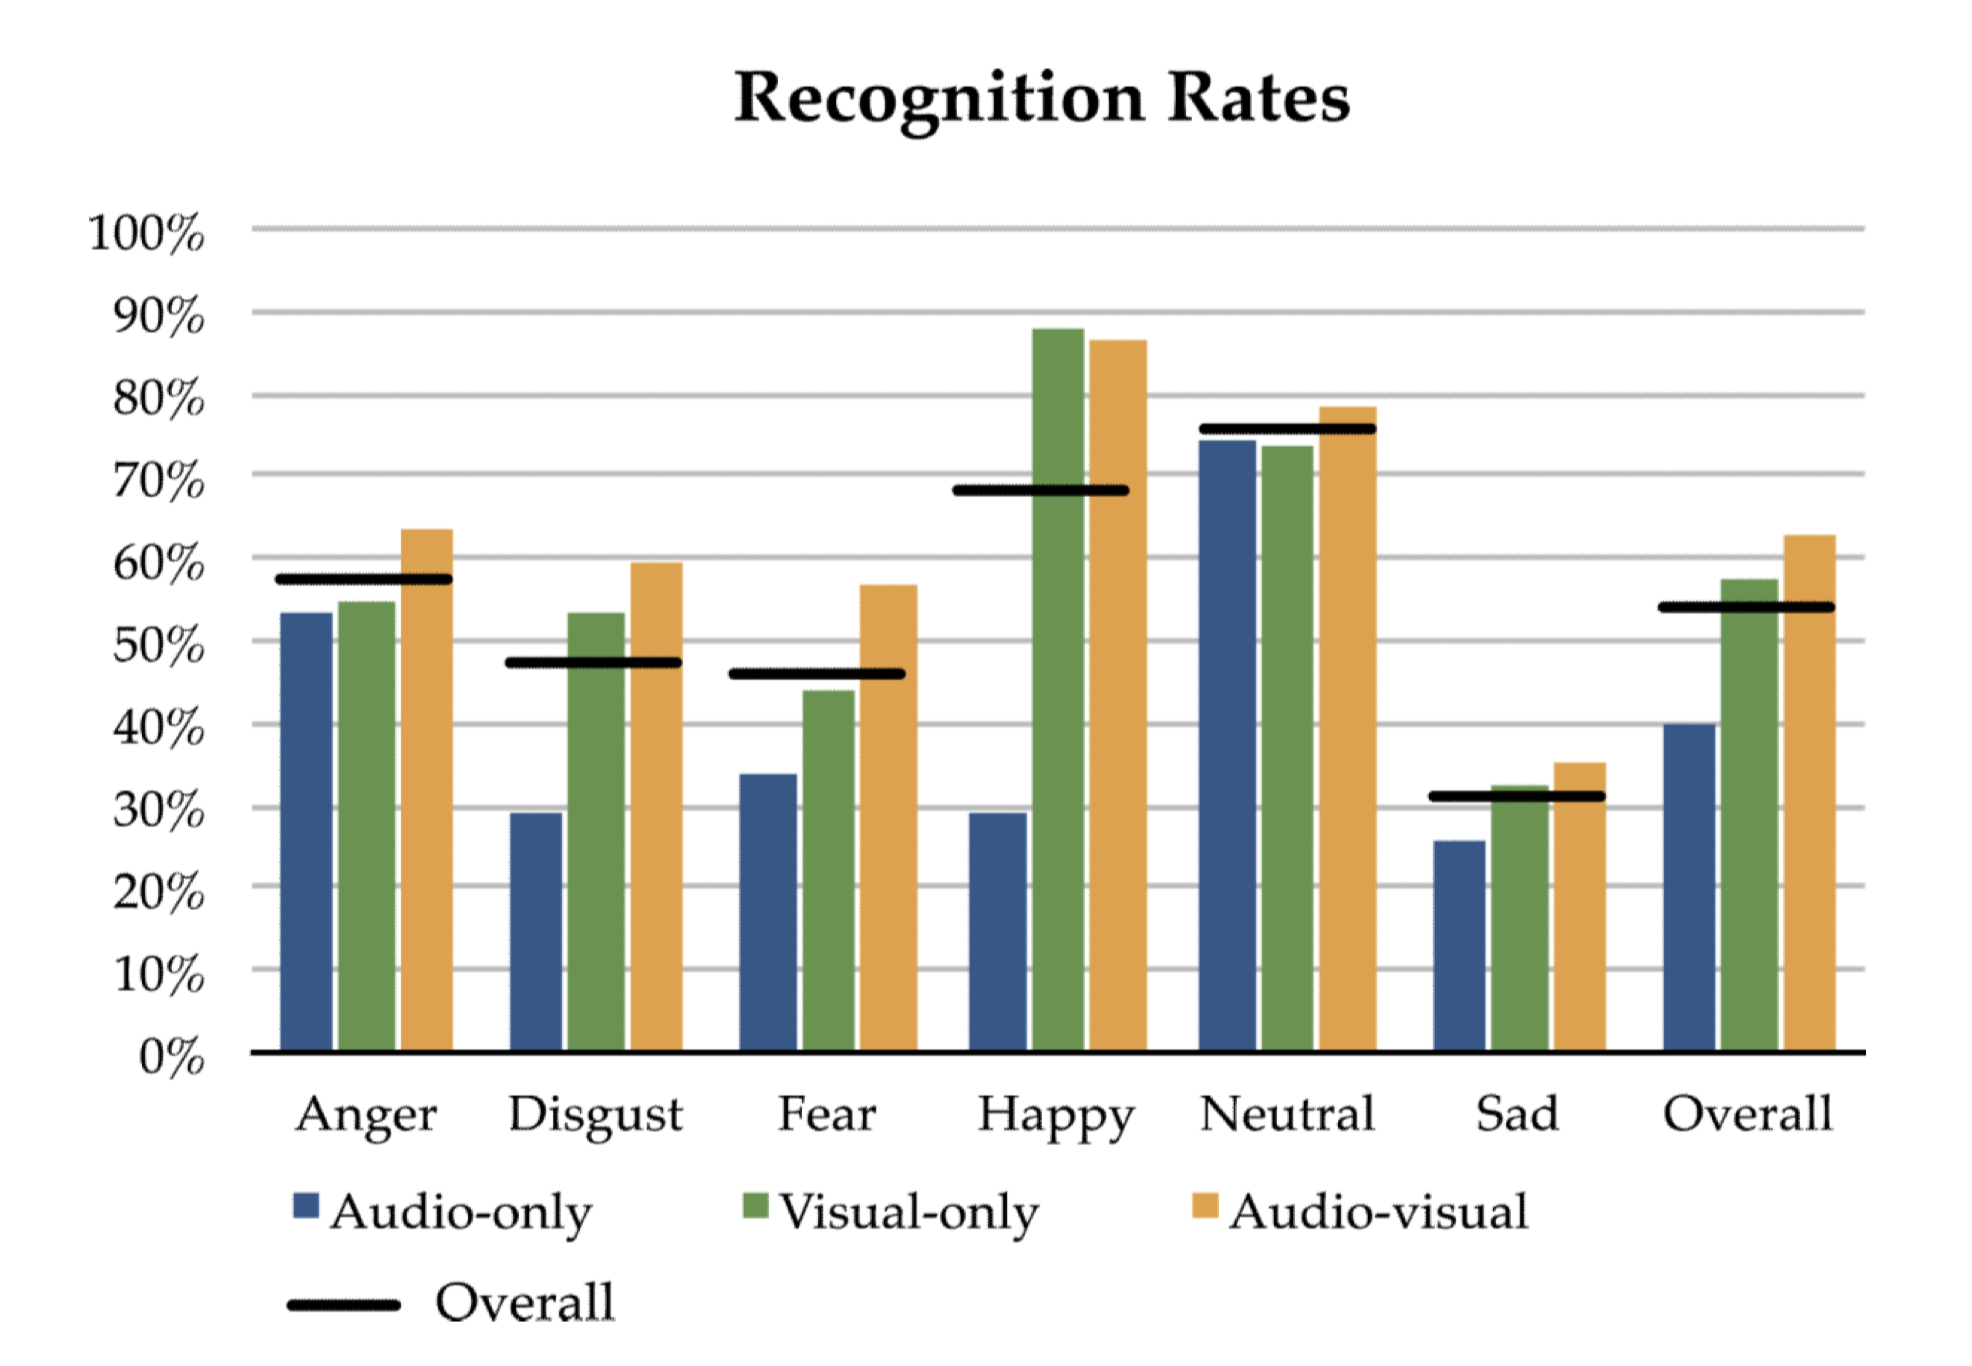
\includegraphics[width=0.8\textwidth]{res/crema.png}
    \caption{The results of the human annotation on the CREMA-D corpus \cite{cao2014crema}. There generally is a trend for audio-visual videos to be labelled better than visual-only data. There are also differences in accuracy depending on the emotion.}
    \label{fig:crema_results}
\end{figure}

Some questions remain unanswered. How do human annotators perform if they are confronted with still images of people talking? Are there any significant differences in accuracy depending on the phoneme that is spoken in the image? Those questions may help us in constructing a FER model that is robust against speech. 

We will first analyse the performance of existing FER models against speaking subjects. Since our classic FER models are trained on single images, we will use still frames to evaluate them. We then analyse the phonetic bias of the model (Figure \ref{fig:phone_acc_ravdess}). The accuracy of our model differs depending on the phoneme. The best phonemes \texttt{Z} and \texttt{IY0} have accuracies of 49\%, whereas the worst performing phoneme \texttt{AY1} has an accuracy of only 40\%.
%With the help of the MFA (Section \ref{sub:mfa}) we were able to extract frames from the RAVDESS database (Section \ref{sub:ravdess}) with their respective phoneme labels
\begin{figure}
    \centering
    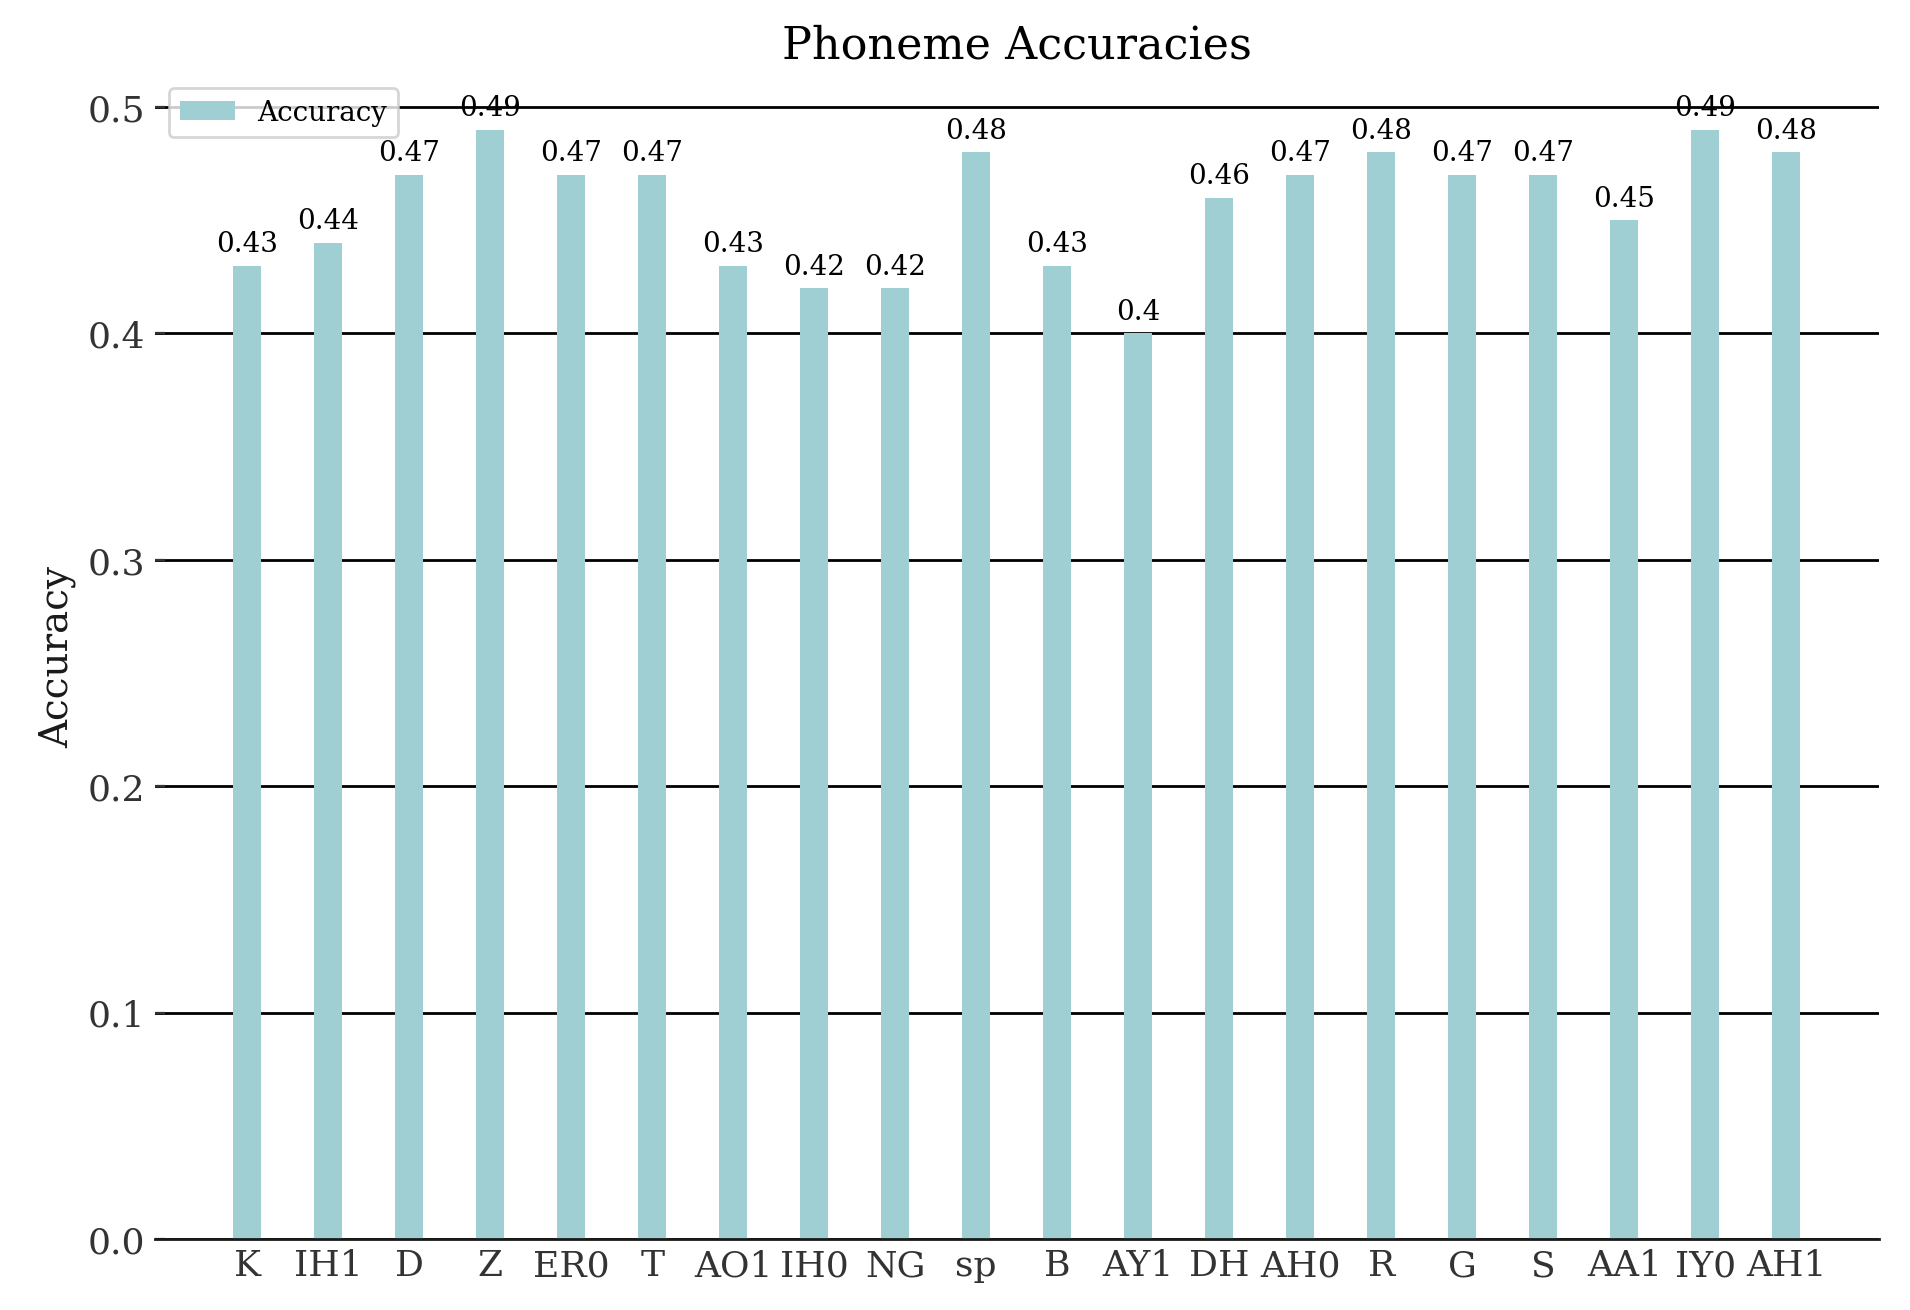
\includegraphics[width=0.8\textwidth]{res/phone_acc_model.png}
    \caption{Accuracies of our classic FER model depending on the phoneme that was spoken in the classified frame. Accuracies range from 40\% to 49\%, showing a significant bias on the spoken phonemes.}
    \label{fig:phone_acc_ravdess}
\end{figure}
\subsection{Goal}
We have seen that our classic FER models perform differently depending on the phoneme. Human annotators have differing performance based on emotions. An analysis on human bias depending on phoneme is however missing. Getting insights into human performance on emotion estimation depending on the spoken phoneme can help us in our task to build FER models that are more robust towards speech.

Is human bias similar to the bias shown in our models? Are humans capable to judge the emotional state of a speaking subject just by looking at a single frame, or does the performance increase when a video (without sound) is available? These are the questions we want to answer in this section.

\subsection{Setup and Material}
We turned to the RAVDESS dataset \cite{livingstone2018ryerson} for the material of our study. Compared to the CREMA-D corpus, RAVDESS also includes the \texttt{surprised} emotion, which will be part of our future models. We want our annotators to label the videos and selected still images from those videos. Given the size of the RAVDESS corpus, we decided to label a subset of the database. Videos of actors 4 (f), 5 (m), 9 (m), and 14 (f) were chosen, with two videos for each of the seven core emotions. The \texttt{calm} emotion was ignored, because it will not be part of our future models since they will follow the seven core emotions from Ekman. This amounts to $4 \cdot 7 \cdot 2 = 56$ videos. To keep the amount of image labels manageable, we chose a subset of phonemes. Our choices were the phonemes \texttt{AY1}, \texttt{Z}, and \texttt{B}. We chose those phonemes because they include some of the best and worst performing phonemes on the model. That way we can later compare the performance of human labellers on those phonemes and draw conclusions on human bias. The total amount of images was 168, with each phoneme being represented 56 times.

To limit faulty annotations due to fatigue at the end of a long labelling session, the data was split into two groups. The first group was labelling videos and images from actors 4 and 5, and the second group was tasked with the data from actors 9 and 14. In total, each group had to label 28 videos and 84 images.

Annotators were first labelled the images before continuing to the videos. Since the images were sourced from the same videos that were labelled we wanted to make sure that there was no bias on the image labels from the perception of the videos.
% This was done to make sure that the labels for the images were not biased by the perception of the videos.

\subsection{Implementation}
The study was done through a simple web application. It was implemented using Svelte for the frontend application, while the data management and hosting was done through firebase. The annotations were saved in real-time, making sure that all completed labels were available in case of connection issues \cite{baur2021}.

Each batch was saved as a document in the Firestore Database. The document included the start time for labelling, the labelled group, a unique identifier, and the image and video selections in two separate dictionaries: 
% https://www.overleaf.com/learn/latex/Code_listing#Reference_guide

\begin{lstlisting}[caption=Data structure of the Firestore document for each labelled batch.] 
{
    createdAt
    group
    id
    imageSelections: {
        imageId: label
    }
    videoSelections: {
        videoId: label
    }
}
\end{lstlisting}

\subsection{Annotators}
The annotators were recruited through personal contacts and a university seminar on a voluntary basis. In total, 16 participants annotated their batches. This leads to each data group being annotated eight times. All annotators were university students in their 20s.

Participants were prepared for the task through a presentation. They were especially told not to take too much time on each datapoint, to make sure that their first impression was determining the respective label.

\subsection{Results}

\paragraph{Temporal Dimension}
The annotators labelled both image and video data. The images are still frames from the videos. This allows us to compare the labelling performance between still frames and videos, and thus judge the importance of a temporal dimension. Our results, as seen in Figure \ref{fig:setting_overview}, conclude that 75.8\% of videos were labelled correctly, whereas the accuracy on the images was only 60.5\% (446 video labels, 1425 image labels). This indicates that temporal data is very advantageous for FER purposes when the subject is talking.


\begin{figure}
    \centering
    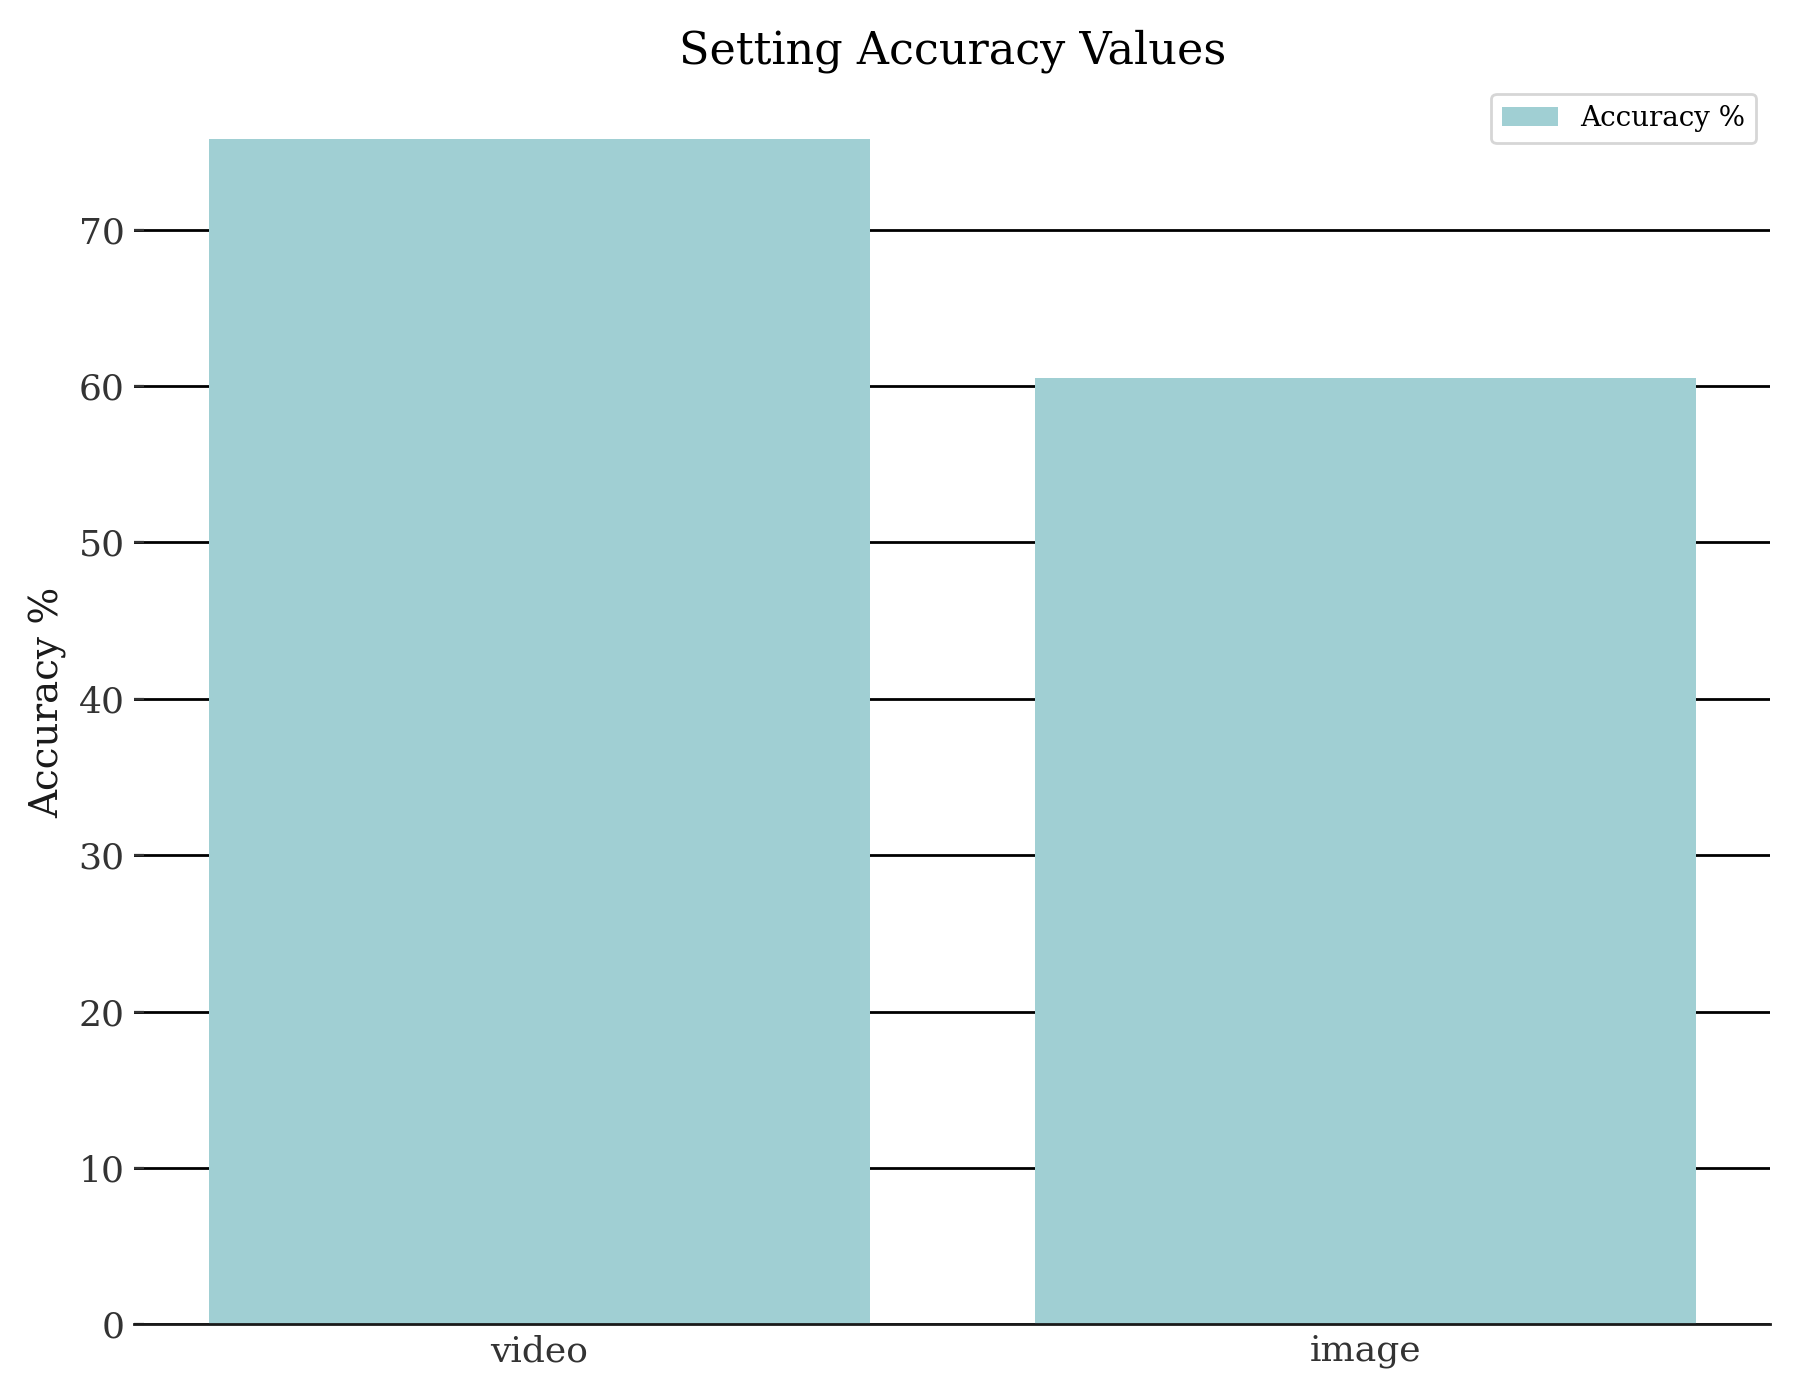
\includegraphics[width=0.65\textwidth]{res/Setting_overview.png}
    \caption{A comparison between the labelling accuracy of image and video data. Video annotation accuracy is considerably higher, leading us to conclude that the temporal dimension is of high importance in FER during speech.}
    \label{fig:setting_overview}
\end{figure}

\paragraph{Lexical Compensation}
The labelled images were chosen on selected phonemes \texttt{AY1}, \texttt{Z}, and \texttt{B}. We can thus compare the annotator's accuracies on the individual phonemes. As seen before, there is a significant difference on the phonemes when our model labelled the images. The human annotators are consistently better, with an accuracy of 60\% across all phonemes. This concludes that humans can compensate for the lexical content (the phonemes), which is something we want to include in our models.

\begin{figure}
    \centering
    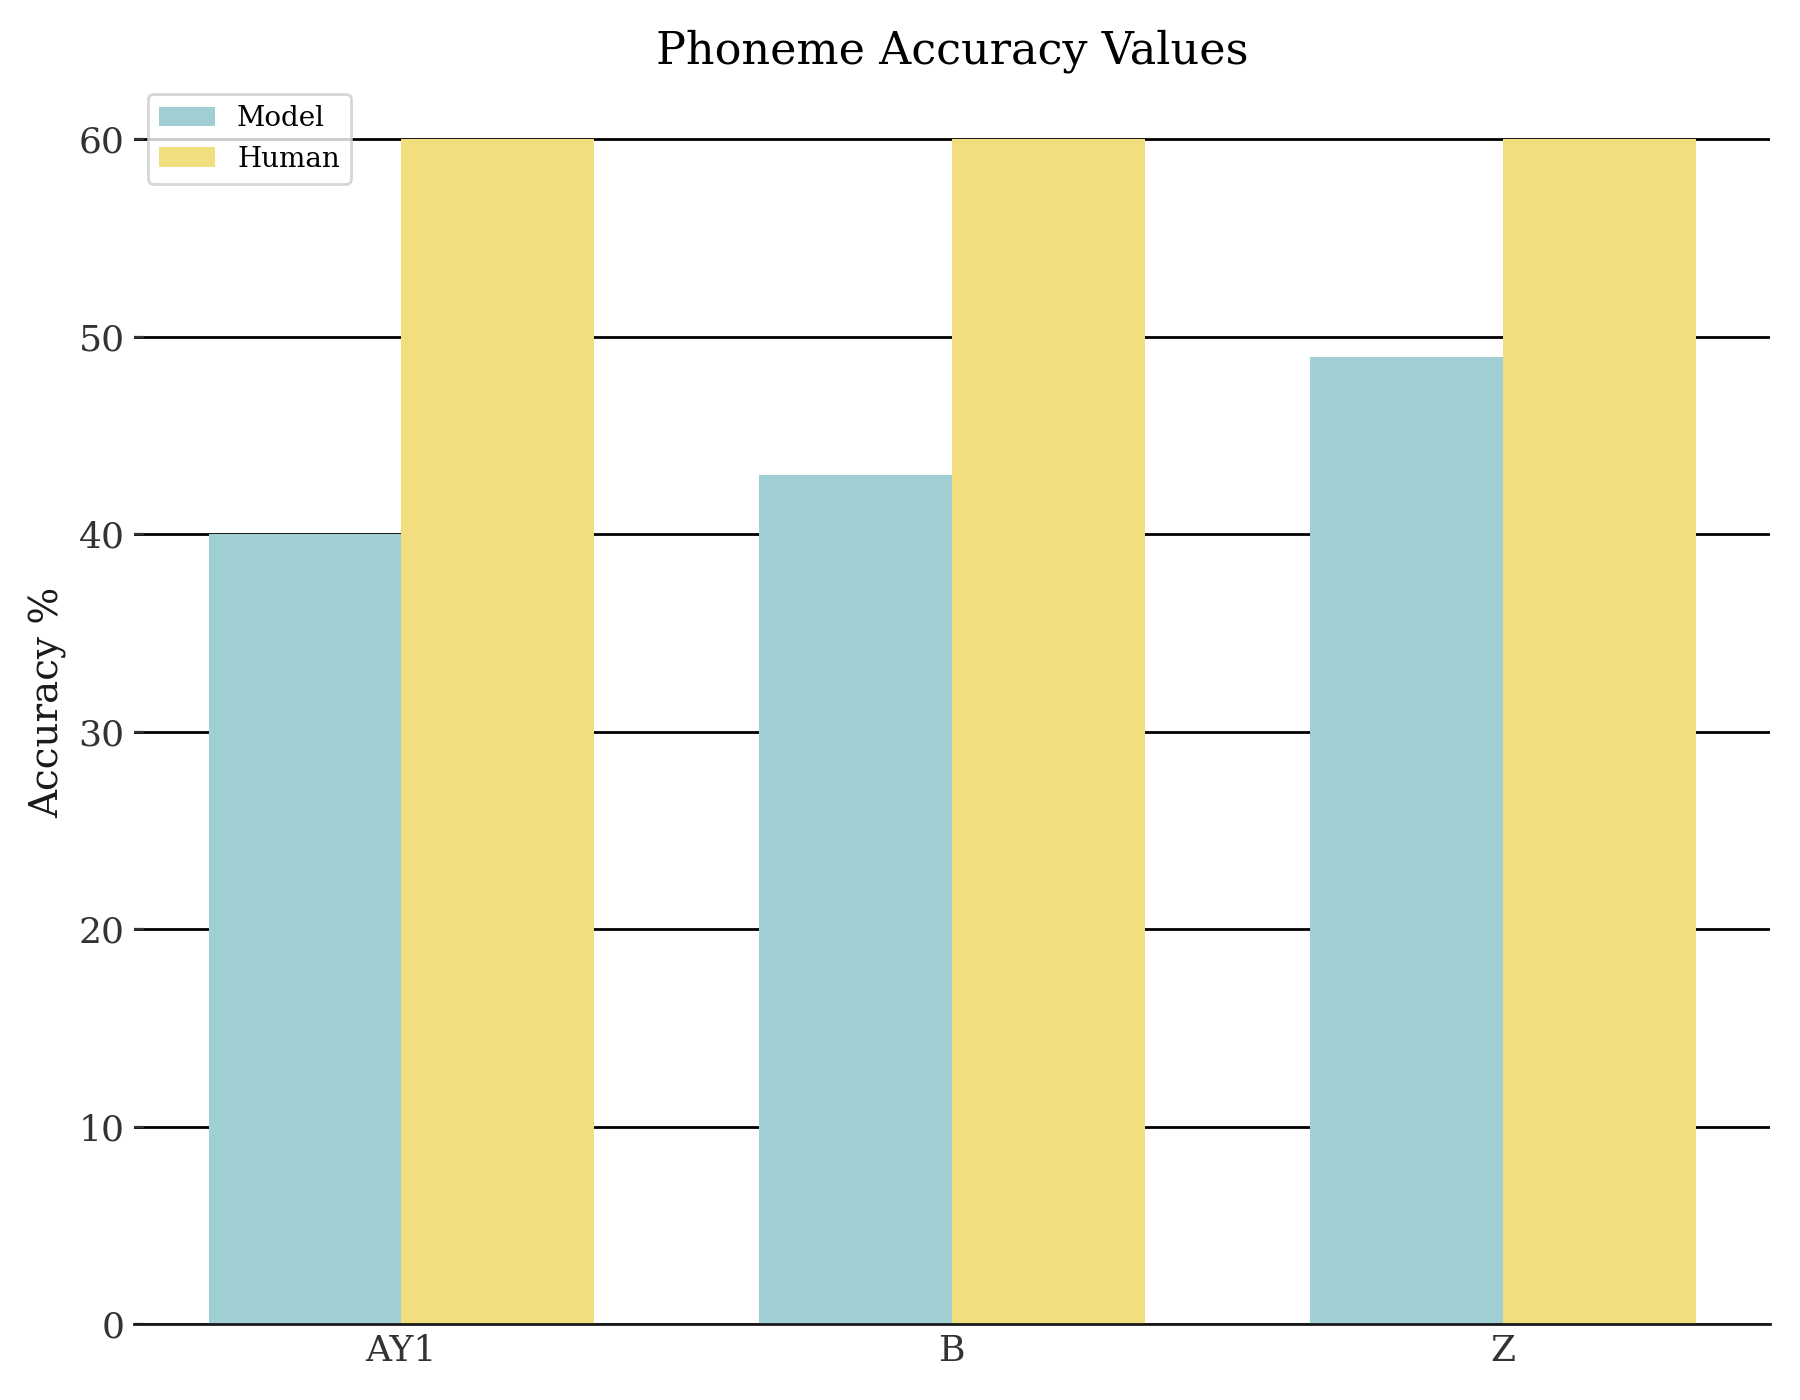
\includegraphics[width=0.65\textwidth]{res/Phone_model_acc.png}
    \caption{A comparison of the accuracies on the individual phonemes from the FER model and human annotators. The latter are better, while also having a consistent accuracy on the phonemes.}
    \label{fig:phone_model_human}
\end{figure}

\paragraph{Further Evaluation}

\section{Building Models on Human Perception}
\label{sec:models}

The previous section has yielded interesting results from human labelling (Section \ref{sec:human}). We concluded that a temporal dimension, and a lexical compensator might help in improving existing FER models for speaking subjects. 

Our current FER models are working on static images, which means that we will have to temporalize them in some way. We will discuss this in section \ref{sub:temp}. A lexical compensator will have to be done with a separate model. There are different approaches to this, as we have seen in section \ref{sec:existing}. We will discuss this in section \ref{sub:lex}.


\subsection{Temporal Dimension}
\label{sub:temp}
As discussed previously, we want to keep and build on existing FER models. Given that some of our models will work on video data, we will have to temporalize our models which currently work on static images.

The straight forward approach is to take the current model, and wrap it in a temporal layer. This means that an input video with 60 frames will produce 60 output embeddings, which can then be fed into a recurrent layer like a LSTM or GRU. This produces minimal overhead, while preserving all weights from our model.

We will use this approach in all our upcoming models.

To have a comparison between frame sizes and an estimation of the importance of the temporal dimension, our models were trained on 1, 30, 60, and 90 frames.

\begin{figure}
    \centering
    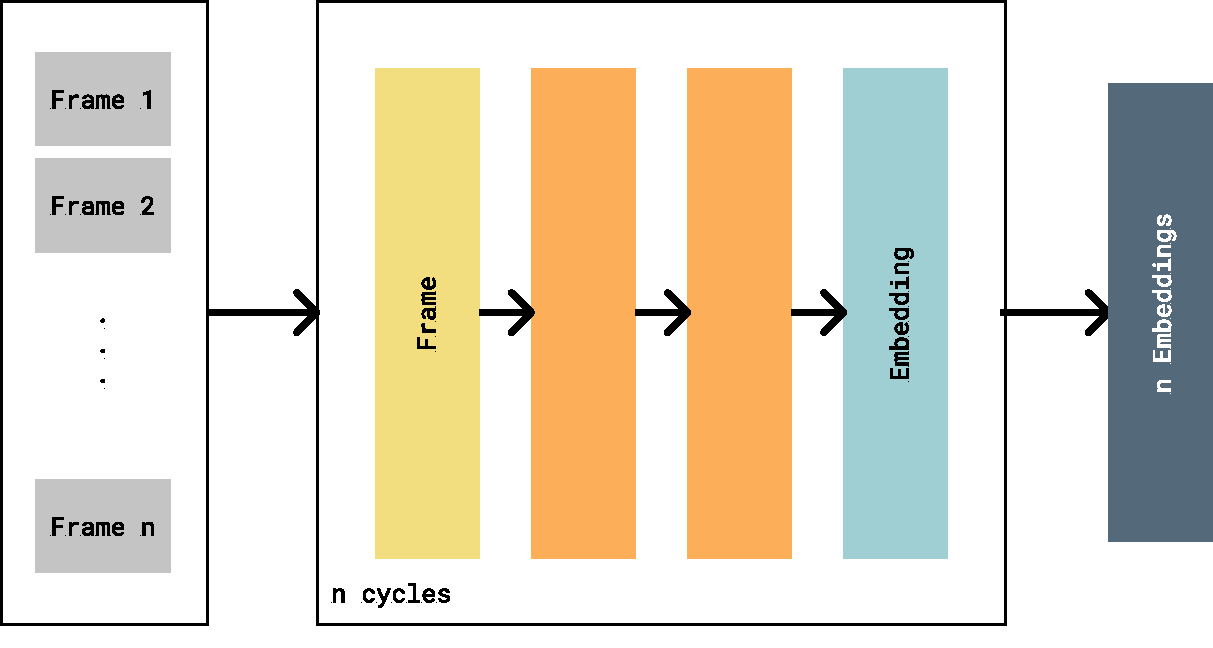
\includegraphics[width=0.8\textwidth]{res/temporalization.pdf}
    \caption{Temporalizing an FER model. The existing model gets wrapped in a TimeDimensional layer. That way the model produces $n$ embeddings for $n$ inputs.}
    \label{fig:temporalization}
\end{figure}

\subsection{Lexical Compensators}
\label{sub:lex}
Lexical compensators can come in different shapes and forms. We will focus on the two previously mentioned approaches from Bursic \cite{bursic2020improving} and Busso \cite{salman2020style}, which attempt to extract lexical information in different ways.

\paragraph{LipNet} 
Bursic et al. \cite{bursic2020improving} used a LipNet embedding to detect the lexical content. We reproduced their approach to analyse the performance of the architecture, using our own MobileNet. The dataset of choice, similarly to the original model, was RAVDESS. The validation data consisted of all the recordings of actors 4, 5, 9, and 14.

\paragraph{Style Extractor}
The lexical compensator of Salman and Busso \cite{salman2020style} served as the inspiration for our own. However, we made some changes to the architecture and preprocessing of the style extractor. We turned to FaceMesh as a facial landmark detector, yielding 468 three-dimensional coordinates, 1404 inputs in total. We chose a smaller, non temporal architecture network, with only one hidden layer.

We trained several different models to optimize the size of the style extractor. Given that a hidden layer of 3000 neurons overtrained the model, we drastically stepped down to 512, 256, and 128 neurons. The validation loss of the model was chosen as the deciding metric. 
All three smaller models generalized well with a very similar validation loss. We ultimately continued with the smallest models, yielding a more compact model.

Another difference to the original approach was our decision to remove the second, unused output which predicts the underlying phoneme. Several test runs using a phoneme output yielded no improvement on the actual style extractor output.

The dataset used to train this model, like in the original paper, was CREMA-D.

\begin{figure}
    \centering
    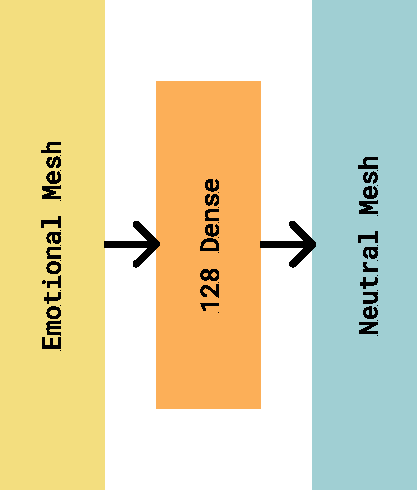
\includegraphics[width=0.5\textwidth]{res/FExtractor.pdf}
    \caption{The architecture of our final feature extractor. The emotional input mesh of a subject speaking a given phoneme $p$ gets passed to a densely connected hidden layer with 128 neurons. The output of the network is a prediction of a neutral mesh of the actor pronouncing the same phoneme $p$.}
    \label{fig:fextractor}
\end{figure}

\subsection{Building the Models}

To complete the architecture, we will breifly talk about the the fusion layers. In instances where two model inputs come together (e.g. the lexical compensators) we need a network that combines both inputs. We want this fusion network to be consistent across all our models to make sure that differences in results are not due to differing architectures.

We turned to the fusion layer by Bursic et al. \cite{bursic2020improving}. We already try to replicate their approach with the lexical compensation from LipNet, and our FER model has a similar embedding with 512 neurons to their VGG19 model. This lets us better compare our results to theirs. In comparison to the model from Salman and Busso \cite{salman2020style}, this fusion network covers all seven core emotions.

To judge the impact of the lexical compensators we also trained a model that only uses the temporalized embedding of our FER model. We use the same fusion network, this time in a transfer learning approach. The FER embedding of 512 neurons gets passed to the same fusion network, foregoing the \texttt{concatenate} step. This aides in comparing the impact of the lexical compensators without having any noise from a differing transfer network.

The input from the previous model(s) are fed into a bidirectional GRU layer of size 256. A dense layer of size 16 follows. The final output layer is a densely connected layer of size 7, corresponding to the core emotions. The activation function of the hidden layers are ReLU, while the output layer has a softmax activation function. A dropout layer of 0.5 is placed between the GRU and the following dense layer (see Figure \ref{fig:fusionlayers}).

We end up with three main architectures:

\begin{enumerate}
    \item \textbf{Temporal FER model} The temporalized FER model without a lexical compensator.
    \item \textbf{Lexical compensation with LipNet} The temporalized FER model with LipNet as the lexical compensator.
    \item \textbf{Lexical compensation with our style extractor} The temporalized FER model with a self trained style extractor as the lexical compensator.
\end{enumerate}

\begin{figure}
    \centering
    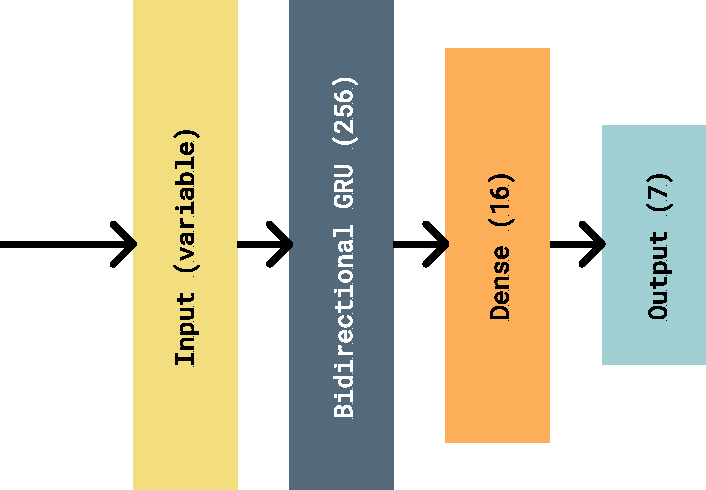
\includegraphics[width=0.7\textwidth]{res/FusionLayers.pdf}
    \caption{The architecture of the fusion/transfer network. It is kept simple to accommodate the smaller datasets we use and follows the architecture from Bursic et al. \cite{bursic2020improving}.}
    \label{fig:fusionlayers}
\end{figure}
\subsection{Data and Preprocessing}
\paragraph{Data for FER Models}
We mainly use two datasets in our work, RAVDESS and CREMA-D. Since the actual usage of the data is dependent on some preprocessing steps like face-/mouth-cropping and landmark extraction, we transformed the datasets before starting the training cycles on them.

The FER-model takes a facial crop of the frame, with 224x224x3 dimensions (width, height, colour channels). In preprocessing, we saved a crop of every frame for all videos. 
The LipNet model needs a 100x50x3 dimensional input of the orofacial area. This crop is saved alongside the facial crop for each frame. Both the facial and orofacial crops were done with the frontal face detector of dlib \cite{dlib09}.

Finally, our lexical compensator will be trained on facial landmarks extracted from FaceMesh. Those are also stored with the facial and orofacial crops.

Each videos data is saved as an array in a \texttt{pickle} file. The structure of the file can be seen in figure \ref{fig:pickle}.
\begin{figure}
    \centering
    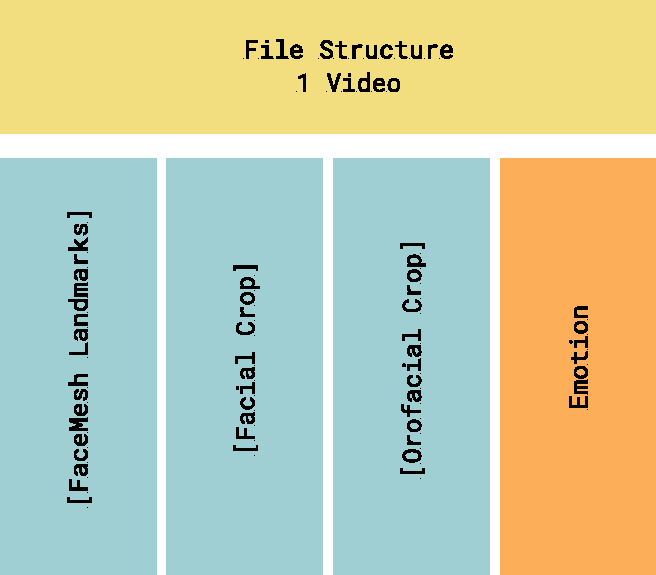
\includegraphics[width=0.5\textwidth]{res/Pickle.pdf}
    \caption{The data structure of our preprocessed files. Each file corresponds to one video. Its facial and orofacial crops, alongside with its facial landmarks are stored in arrays. The array lengths correspond to the amount of frames in each video. The underlying emotion is saved as well.}
    \label{fig:pickle}
\end{figure}

\paragraph{Data for the Style Extractor}
To be able to train the style extractor we need pairs of meshes for every phoneme, where one mesh was emotional (not neutral) and one neutral. To have a more fine-grained model, we also wanted to make sure that all mesh pairs are from the same occurrence. As an example, the sentence "It's eleven \textbf{o}'cl\textbf{o}ck" has two occurrences of the phoneme \texttt{O} (marked). When training the style extractor, all mesh pairs came from the same actor in the same sentence at similar positions.


\subsection{Training}
Here we present some more detailed information for the training process of our models.
\paragraph{General Information}
To keep the models comparable on the temporal dimension, we trained each model on 1, 30, 60, and 90 frames. The FER and LipNet model were pre-trained and locked. We wanted to cover the core emotions that were defined by Ekman, and thus ignored the \texttt{calm} emotion that was provided by the RAVDESS dataset.

To get the most out of each video, we used a sliding window approach on the frame arrays. Given a model with a frame size of 60 and a video with 100 frames, we now have the opportunity to extract multiple data point from the video. We used a window stride of 5. This means that the first data point ranges from frame 0 to 59, the second from 5 to 64 and so on. This helped to somewhat ease the problem of the RAVDESS dataset being too small for proper DNN training. 

Our specific feature extractor was trained separately. It was trained on CREMA-D, with actors 1 to 11 being used for validation.

The fusion networks for all models was trained on RAVDESS. Actors 4, 5, 9, and 14 were used for the validation set, the files from the other 20 actors were used for training.

\paragraph{Technical Details}
We used the \texttt{keras} environment using a \texttt{tensorflow} backend (version 2.4.1) to train our models on a HPC using an Nvidia Titan X GPU with the Pascal architecture. The scripts were deployed in Docker containers, on a server running Ubuntu 18.04 LTS.

\subsection{Results}
In this chapter we will present the results of our training. More detailed results and discussion can be found in section \ref{sec:discussion}.

\newpage
\section{The Impact of Language and Improvisation}
\label{sec:data}
Training and validating models for research is usually done on the same dataset. This leads to solid proof-of-concept models, but can produce models that do not generalize well to real world scenarios. 

Another aspect of robustness of FER models against speech, which is the language dimension. We want to provide a platform to test our models against a different language, to see if this modality impacts performance. In this section we will present our approach to build a small database in German along the lines of RAVDESS. The datasets we used in this thesis are all recorded in English, and by comparing the performance of the models on the German recordings we can gain insights into their language dependency (Section \ref{sec:multilingual}). 

Another point to note is that the datasets we used are scripted and acted. Real world situations are not as rigid and more closely follow speech acts. We also collect videos of speech-acts that more closely resemble those of real world scenarios to later validate our models on them.

\subsection{Recording Setup}
We used the TAWNY recording tool \cite{tawny2021} for data collection. Each database was set up in a separate project. The participants recorded the videos themselves from home. Each recording was preceded with an information card (Figure \ref{fig:infocards}) which described the task for each video. The participants were given time to prepare their statements and could start their recording at their chosen time. Since the participants had to record themselves through a web browser application, the quality of videos varied depending on the available equipment.

\begin{figure}
    \centering
    \begin{subfigure}[b]{0.45\textwidth}
      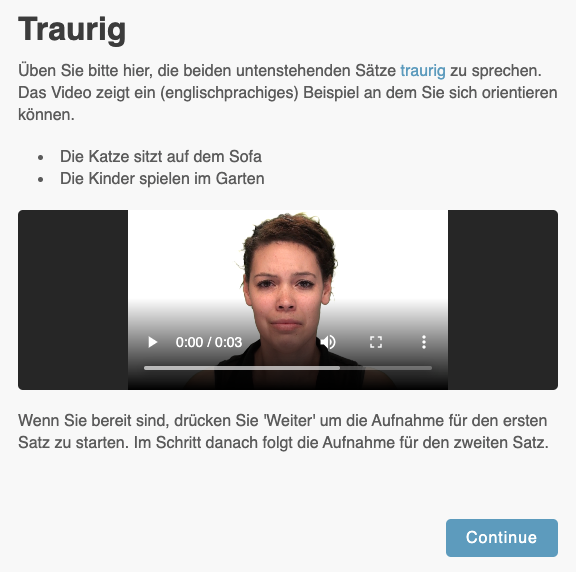
\includegraphics[width=\textwidth]{res/ger_ex.png}
    \end{subfigure}
    \begin{subfigure}[b]{0.45\textwidth}
      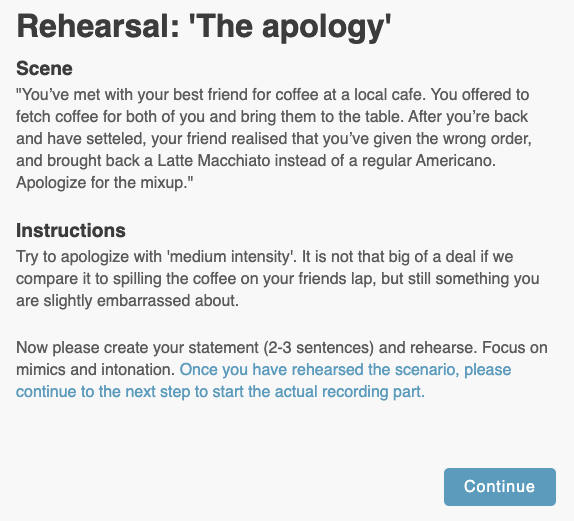
\includegraphics[width=\textwidth]{res/impro_ex.png}
    \end{subfigure}
    
    \caption{Information cards for each database project (Left: German RAVDESS, Right: Real World Speech Acts). The cards described the task for the following recording.}
    \label{fig:infocards}
\end{figure}

The videos were stored on the TAWNY platform \cite{tawny2021platform}, a SaaS emotion analytics platform, and were available for download after the participant concluded the recording of the given task.

\subsection{German RAVDESS - GRD}
\label{sec:german}

The lexical content of RAVDESS is kept simple. The actors speak two easy to pronounce sentences in eight emotions. We replicate this by switching the English sentences for German counterparts. We chose the two neutral statements "Die Katze sitzt auf dem Sofa" and "Die Kinder spielen im Garten", two sentences with eight syllables and commonly used words. The emotions are the same as in the RAVDESS database: neutral, calm, happy, sad, angry, fearful, surprise, and disgust.

Recordings were done using the TAWNY recording tool \cite{tawny2021}. The actors were given a general description of the task before starting their session. Before each individual recording the actors were given the target sentence and emotion, alongside an example from the RAVDESS dataset. The recordings were split, as the actors recited one statement per take. 

14 actors participated, 8 female and 6 male. We checked the videos for visual quality and sufficient emotional perception. After quality assessment, we end up with 141 recordings from 11 actors.

\subsection{Real World Speech Acts}
\label{sec:rwsa}
We want to figure out the impact of real world speech acts on our models and the emotional state of subjects. Compared to other datasets we use, the recordings in this collection do not have an underlying emotion. The emotional state should be induced by the statement and situation itself rather than from a scripted and ordered statement.

To collect statements that fit in real world scenarios, we put the actors in situations where they had to react with their own words. Four scenarios were built to produce certain responses:

\begin{enumerate}
    \item \textbf{Promise} "Together with one of your coworkers, you have just finished your lunch at a local restaurant. When it is time to pay, you realise that you forgot your wallet at the office. Knowing how stingy your colleague can be, try to ask him if you could borrow some money and affirm that you will give it back once you’re back at work."
    \item \textbf{Order} "You are the team lead of the sales team. You currently have the weekly meeting with your team members. Given that the yearly report is about to be due, it’s a very important week ahead. Remind Thomas that he is in charge of creating the final draft of the report, and tell him that it is due until next Friday."
    \item \textbf{Apology} "You’ve met with your best friend for coffee at a local cafe. You offered to fetch coffee for both of you and bring them to the table. After you’re back and have settled, your friend realised that you’ve given the wrong order, and brought back a Latte Macchiato instead of a regular Americano. Apologize for the mixup."
    \item \textbf{Assessment} "You are the team lead of the sales team. After a long and busy week, you meet with your team members for a debrief. Thomas has done a great job on the final draft of the yearly report, which he handed in on time. Compliment him on his great work."
\end{enumerate}

The recordings were collected with the TAWNY recording tool \cite{tawny2021}. The actors were confronted with the situation, and had time to make up a response before being recorded. Five people participated, one male and four female. After quality assessment, the recordings of only four participants were deemed usable. This is unfortunately not enough for detailled analysis.

\subsection{Discussion}
\label{sec:data_discussion}
\subsubsection{Multilingual Performance}
\label{sec:multilingual}
We validated our models on the videos of the GRD dataset from section \ref{sec:german}. The models for 90 frames could not be used since the videos were too short. The general trend from section \ref{sec:cross_dataset} is confirmed. The FER-TC model and the FER-SE model perform increasingly better with higher frame-window size. The FER-LN models performance does not increase with more temporal information. Compared to the results from section \ref{sec:cross_dataset} there is another decrease in accuracy, of around 10 percentage points. It is however not conclusive if this decrease is due to the language switch or other factors:
\begin{itemize}
    \item The recordings are not of the same quality as those of CREMA-D. For practical reasons all recordings had to be done remotely by the actors themselves using the TAWNY recording tool.
    \item The preparation of the actors were not comparable to those on CREMA-D. We did not have stimuli to actually put the actors into the desired emotional state and relied on their acting ability to convey the emotion.
    \item The actors only had one take to record their statements. Producers of other datasets generally have the capacity to have multiple takes for each recording.
\end{itemize}

\begin{figure}
    \centering
    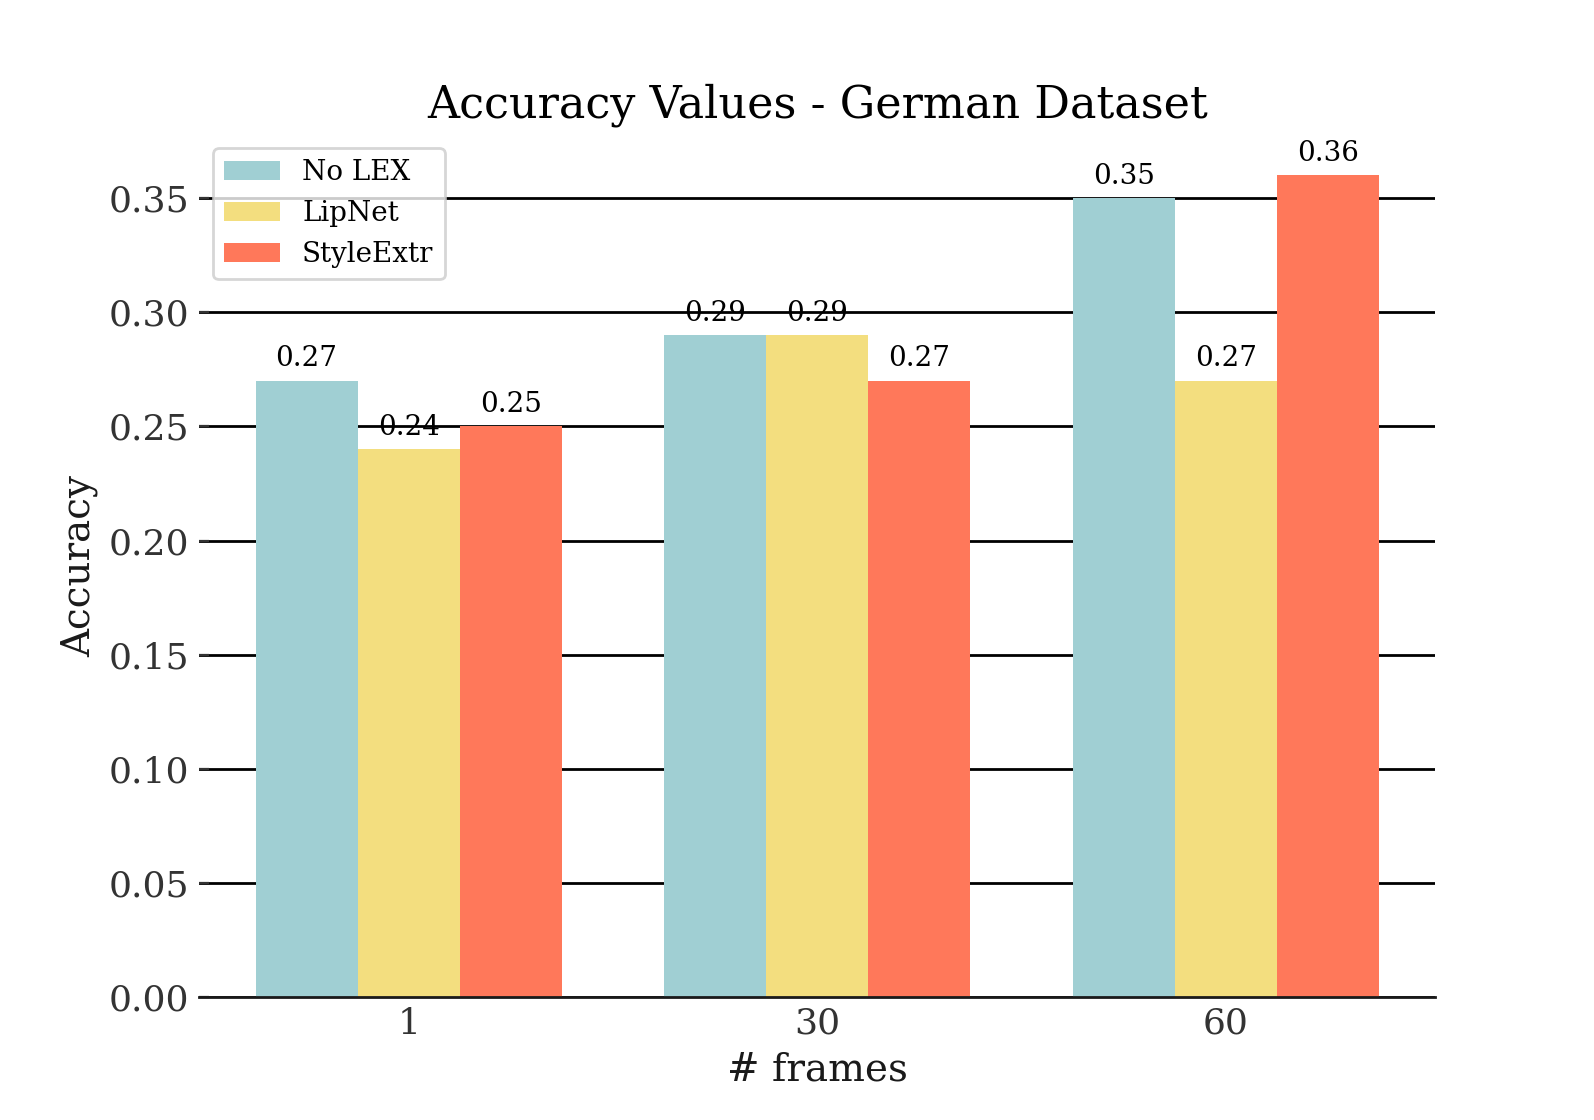
\includegraphics[width=0.8\textwidth]{res/GermanResults.png}
    \caption{Evaluating the models we trained on the GRD dataset from section \ref{sec:german}.}
    \label{fig:german_res}
\end{figure}

We can conclude that our models can adapt to recordings in German without much trouble. We would expect to see usable and comparable results with a dataset of another language given similar quality.

\subsubsection{Improvised Data}
The data collected in section \ref{sec:rwsa} was not extensive enough to provide any evaluation. Nevertheless we want to discuss the possibilities for analysis and our collection method.

We collected the data remotely with the TAWNY recording tool. The stimuli that described the scenarios (Section \ref{sec:rwsa}) were given in text form, and the actors had time to prepare their responses. Given that we want an improvised reaction that is not scripted, we suggest that the setup and introduction to the scenario should rather be given in a sketched video to immerse the actor into the situation. The response should also be given immediately without any time to prepare the statement.

To analyse the recordings, we would first need labels for the recordings. Since the statements were not induced by a predefined emotion, the labels would have to be manually added in postprocessing by human annotators. Since its possible that there are several emotional states during one recording, we would have the ability to detect and evaluate emotional shifts during speech, and analyse how our models cope with them. 
% \chapter{Conclusions}
\section{Discussion}
\label{sec:discussion}
\section{Conclusion}

%______________________________________________________________________

\cleardoublepage
\fancyhead[LE,RO,LO,RE]{} % Keine Kopfzeile mehr oben auf jeder Seite
\section*{Inhalt der beigelegten CD}
%______________________________________________________________________

\cleardoublepage
\printbibliography

\end{document}
